\documentclass[11pt, a4paper]{article}
% =============================================================
%  preamble.tex — Reusable preamble for Neural Networks course
%  Usage: % =============================================================
%  preamble.tex — Reusable preamble for Neural Networks course
%  Usage: % =============================================================
%  preamble.tex — Reusable preamble for Neural Networks course
%  Usage: \input{preamble} at the top of your document,
%         after \documentclass but before \begin{document}.
% =============================================================

% --- Encoding & language ---
\usepackage[T1]{fontenc}
\usepackage[utf8]{inputenc}
\usepackage[english]{babel}         % swap for [french] if needed

% --- Page geometry ---
\usepackage{geometry}
\geometry{top=2.5cm, bottom=2.5cm, left=2.5cm, right=2.5cm}

% --- Math ---
\usepackage{amsmath, amssymb}

% --- Tables ---
\usepackage{booktabs}               % \toprule, \midrule, \bottomrule
\usepackage{array}                  % column type extensions
\usepackage{tabularx}               % auto-width columns
\usepackage{multirow}               % multi-row cells

% --- Colors ---
\usepackage{xcolor}

\definecolor{mainblue}{RGB}{30, 80, 160}
\definecolor{lightblue}{RGB}{220, 235, 255}
\definecolor{accentgray}{RGB}{245, 246, 248}
\definecolor{darkgray}{RGB}{80, 80, 80}
\definecolor{solutiongreen}{RGB}{20, 120, 60}
\definecolor{lightgreen}{RGB}{220, 245, 230}
\definecolor{warnorange}{RGB}{210, 120, 20}
\definecolor{lightorange}{RGB}{255, 243, 220}

% --- Lists ---
\usepackage{enumitem}

% --- TikZ & pgfplots ---
\usepackage{tikz}
\usepackage{pgfplots}
\pgfplotsset{compat=1.18}
\usetikzlibrary{positioning, arrows.meta, calc, patterns}

% --- Boxes: tcolorbox ---
\usepackage{tcolorbox}
\tcbuselibrary{skins, breakable}

% Generic exercise box (blue border, gray background)
\tcbset{
  exercisebox/.style={
    enhanced,
    colback=accentgray,
    colframe=mainblue,
    boxrule=0.8pt,
    arc=4pt,
    left=10pt, right=10pt, top=8pt, bottom=8pt,
    fonttitle=\bfseries\color{mainblue},
  }
}

% Solution box (green, used in answer sheets)
\tcbset{
  solutionbox/.style={
    enhanced,
    colback=lightgreen,
    colframe=solutiongreen,
    boxrule=0.8pt,
    arc=4pt,
    left=10pt, right=10pt, top=8pt, bottom=8pt,
    fonttitle=\bfseries\color{solutiongreen},
  }
}

% Answer highlight box (orange, for final numeric answers)
\tcbset{
  answerbox/.style={
    enhanced,
    colback=lightorange,
    colframe=warnorange,
    boxrule=0.7pt,
    arc=4pt,
    left=8pt, right=8pt, top=5pt, bottom=5pt,
    fonttitle=\bfseries\color{warnorange},
  }
}

% Step box (light blue border, gray background, for intermediate steps)
\tcbset{
  stepbox/.style={
    enhanced,
    colback=accentgray,
    colframe=mainblue!40,
    boxrule=0.5pt,
    arc=3pt,
    left=8pt, right=8pt, top=6pt, bottom=6pt,
  }
}

% --- Inline note / warning box (mdframed) ---
\usepackage{mdframed}
\newmdenv[
  linecolor=warnorange,
  backgroundcolor=orange!5,
  roundcorner=4pt,
  innerleftmargin=8pt,
  innerrightmargin=8pt,
  innertopmargin=6pt,
  innerbottommargin=6pt,
  linewidth=0.7pt
]{notebox}

% --- Section formatting ---
\usepackage{titlesec}

% Section style: "Exercise N : Title" with a blue rule underneath
% Change the prefix via \renewcommand{\sectionprefix}{...} before \section
\newcommand{\sectionprefix}{Exercise}
\titleformat{\section}[block]
  {\large\bfseries\color{mainblue}}
  {\sectionprefix~\thesection\,:}{0.6em}{}
  [\vspace{-0.3em}\textcolor{mainblue}{\rule{\linewidth}{0.8pt}}]
\titlespacing{\section}{0pt}{1.6em}{0.8em}

% --- Header / Footer ---
\usepackage{fancyhdr}
\pagestyle{fancy}
\fancyhf{}
\renewcommand{\headrulewidth}{0.4pt}

% Customise these three commands in your document after \input{preamble}:
%   \renewcommand{\doccoursename}{My Course}
%   \renewcommand{\docsessionname}{Session N — Topic}
\newcommand{\doccoursename}{Neural Networks for Engineers}
\newcommand{\docsessionname}{Session}

\fancyhead[L]{\small\textcolor{darkgray}{\doccoursename}}
\fancyhead[R]{\small\textcolor{darkgray}{\docsessionname}}
\fancyfoot[C]{\small\textcolor{darkgray}{\thepage}}

% --- Title block macro ---
% Usage: \maketitleblock{Title line}{Subtitle / metadata line}{background color}
% Examples:
%   \maketitleblock{Session 4 — Exercises}{Mixed level | Neural Networks}{mainblue}
%   \maketitleblock{Session 4 — Solutions}{Perceptrons and MLPs | Neural Networks}{solutiongreen}
\newcommand{\maketitleblock}[3]{%
  \begin{tcolorbox}[
    enhanced,
    colback=#3,
    colframe=#3,
    arc=6pt, boxrule=0pt,
    left=16pt, right=16pt, top=12pt, bottom=12pt
  ]
    {\large\bfseries\color{white} #1}\\[4pt]
    {\small\color{white!85!black} #2}
  \end{tcolorbox}
  \vspace{1em}
}

% --- Convenience macros ---

% Blank answer field (inline underline for fill-in tables)
\newcommand{\acell}{\rule{1.8cm}{0.4pt}}

% Step-by-step computation display: \step{label}{math}
% Example: \step{Hidden layer}{z^{(1)} = Wx + b = \ldots}
\newcommand{\step}[2]{%
  \noindent\textbf{#1:}\quad $#2$\par\vspace{0.3em}
}

% Neuron style for TikZ diagrams (reuse with \node[neuron])
% Colors are overridable per layer — see examples below.
%
% Input neuron  : fill=lightblue,  draw=mainblue
% Hidden neuron : fill=green!15,   draw=green!50!black
% Output neuron : fill=orange!15,  draw=orange!70!black
%
% Example architecture diagram:
%
%   \begin{tikzpicture}[
%     neuron/.style={circle, minimum size=1cm, thick, font=\small\bfseries},
%     arr/.style={->, >=Stealth, thick, gray!70}
%   ]
%     \node[neuron, fill=lightblue,  draw=mainblue]          (x1) at (0, 1)  {$x_1$};
%     \node[neuron, fill=green!15,   draw=green!50!black]    (h1) at (3, 1)  {$h_1$};
%     \node[neuron, fill=orange!15,  draw=orange!70!black]   (y)  at (6, 1)  {$\hat{y}$};
%     \draw[arr] (x1) -- (h1);
%     \draw[arr] (h1) -- (y);
%   \end{tikzpicture}
 at the top of your document,
%         after \documentclass but before \begin{document}.
% =============================================================

% --- Encoding & language ---
\usepackage[T1]{fontenc}
\usepackage[utf8]{inputenc}
\usepackage[english]{babel}         % swap for [french] if needed

% --- Page geometry ---
\usepackage{geometry}
\geometry{top=2.5cm, bottom=2.5cm, left=2.5cm, right=2.5cm}

% --- Math ---
\usepackage{amsmath, amssymb}

% --- Tables ---
\usepackage{booktabs}               % \toprule, \midrule, \bottomrule
\usepackage{array}                  % column type extensions
\usepackage{tabularx}               % auto-width columns
\usepackage{multirow}               % multi-row cells

% --- Colors ---
\usepackage{xcolor}

\definecolor{mainblue}{RGB}{30, 80, 160}
\definecolor{lightblue}{RGB}{220, 235, 255}
\definecolor{accentgray}{RGB}{245, 246, 248}
\definecolor{darkgray}{RGB}{80, 80, 80}
\definecolor{solutiongreen}{RGB}{20, 120, 60}
\definecolor{lightgreen}{RGB}{220, 245, 230}
\definecolor{warnorange}{RGB}{210, 120, 20}
\definecolor{lightorange}{RGB}{255, 243, 220}

% --- Lists ---
\usepackage{enumitem}

% --- TikZ & pgfplots ---
\usepackage{tikz}
\usepackage{pgfplots}
\pgfplotsset{compat=1.18}
\usetikzlibrary{positioning, arrows.meta, calc, patterns}

% --- Boxes: tcolorbox ---
\usepackage{tcolorbox}
\tcbuselibrary{skins, breakable}

% Generic exercise box (blue border, gray background)
\tcbset{
  exercisebox/.style={
    enhanced,
    colback=accentgray,
    colframe=mainblue,
    boxrule=0.8pt,
    arc=4pt,
    left=10pt, right=10pt, top=8pt, bottom=8pt,
    fonttitle=\bfseries\color{mainblue},
  }
}

% Solution box (green, used in answer sheets)
\tcbset{
  solutionbox/.style={
    enhanced,
    colback=lightgreen,
    colframe=solutiongreen,
    boxrule=0.8pt,
    arc=4pt,
    left=10pt, right=10pt, top=8pt, bottom=8pt,
    fonttitle=\bfseries\color{solutiongreen},
  }
}

% Answer highlight box (orange, for final numeric answers)
\tcbset{
  answerbox/.style={
    enhanced,
    colback=lightorange,
    colframe=warnorange,
    boxrule=0.7pt,
    arc=4pt,
    left=8pt, right=8pt, top=5pt, bottom=5pt,
    fonttitle=\bfseries\color{warnorange},
  }
}

% Step box (light blue border, gray background, for intermediate steps)
\tcbset{
  stepbox/.style={
    enhanced,
    colback=accentgray,
    colframe=mainblue!40,
    boxrule=0.5pt,
    arc=3pt,
    left=8pt, right=8pt, top=6pt, bottom=6pt,
  }
}

% --- Inline note / warning box (mdframed) ---
\usepackage{mdframed}
\newmdenv[
  linecolor=warnorange,
  backgroundcolor=orange!5,
  roundcorner=4pt,
  innerleftmargin=8pt,
  innerrightmargin=8pt,
  innertopmargin=6pt,
  innerbottommargin=6pt,
  linewidth=0.7pt
]{notebox}

% --- Section formatting ---
\usepackage{titlesec}

% Section style: "Exercise N : Title" with a blue rule underneath
% Change the prefix via \renewcommand{\sectionprefix}{...} before \section
\newcommand{\sectionprefix}{Exercise}
\titleformat{\section}[block]
  {\large\bfseries\color{mainblue}}
  {\sectionprefix~\thesection\,:}{0.6em}{}
  [\vspace{-0.3em}\textcolor{mainblue}{\rule{\linewidth}{0.8pt}}]
\titlespacing{\section}{0pt}{1.6em}{0.8em}

% --- Header / Footer ---
\usepackage{fancyhdr}
\pagestyle{fancy}
\fancyhf{}
\renewcommand{\headrulewidth}{0.4pt}

% Customise these three commands in your document after % =============================================================
%  preamble.tex — Reusable preamble for Neural Networks course
%  Usage: \input{preamble} at the top of your document,
%         after \documentclass but before \begin{document}.
% =============================================================

% --- Encoding & language ---
\usepackage[T1]{fontenc}
\usepackage[utf8]{inputenc}
\usepackage[english]{babel}         % swap for [french] if needed

% --- Page geometry ---
\usepackage{geometry}
\geometry{top=2.5cm, bottom=2.5cm, left=2.5cm, right=2.5cm}

% --- Math ---
\usepackage{amsmath, amssymb}

% --- Tables ---
\usepackage{booktabs}               % \toprule, \midrule, \bottomrule
\usepackage{array}                  % column type extensions
\usepackage{tabularx}               % auto-width columns
\usepackage{multirow}               % multi-row cells

% --- Colors ---
\usepackage{xcolor}

\definecolor{mainblue}{RGB}{30, 80, 160}
\definecolor{lightblue}{RGB}{220, 235, 255}
\definecolor{accentgray}{RGB}{245, 246, 248}
\definecolor{darkgray}{RGB}{80, 80, 80}
\definecolor{solutiongreen}{RGB}{20, 120, 60}
\definecolor{lightgreen}{RGB}{220, 245, 230}
\definecolor{warnorange}{RGB}{210, 120, 20}
\definecolor{lightorange}{RGB}{255, 243, 220}

% --- Lists ---
\usepackage{enumitem}

% --- TikZ & pgfplots ---
\usepackage{tikz}
\usepackage{pgfplots}
\pgfplotsset{compat=1.18}
\usetikzlibrary{positioning, arrows.meta, calc, patterns}

% --- Boxes: tcolorbox ---
\usepackage{tcolorbox}
\tcbuselibrary{skins, breakable}

% Generic exercise box (blue border, gray background)
\tcbset{
  exercisebox/.style={
    enhanced,
    colback=accentgray,
    colframe=mainblue,
    boxrule=0.8pt,
    arc=4pt,
    left=10pt, right=10pt, top=8pt, bottom=8pt,
    fonttitle=\bfseries\color{mainblue},
  }
}

% Solution box (green, used in answer sheets)
\tcbset{
  solutionbox/.style={
    enhanced,
    colback=lightgreen,
    colframe=solutiongreen,
    boxrule=0.8pt,
    arc=4pt,
    left=10pt, right=10pt, top=8pt, bottom=8pt,
    fonttitle=\bfseries\color{solutiongreen},
  }
}

% Answer highlight box (orange, for final numeric answers)
\tcbset{
  answerbox/.style={
    enhanced,
    colback=lightorange,
    colframe=warnorange,
    boxrule=0.7pt,
    arc=4pt,
    left=8pt, right=8pt, top=5pt, bottom=5pt,
    fonttitle=\bfseries\color{warnorange},
  }
}

% Step box (light blue border, gray background, for intermediate steps)
\tcbset{
  stepbox/.style={
    enhanced,
    colback=accentgray,
    colframe=mainblue!40,
    boxrule=0.5pt,
    arc=3pt,
    left=8pt, right=8pt, top=6pt, bottom=6pt,
  }
}

% --- Inline note / warning box (mdframed) ---
\usepackage{mdframed}
\newmdenv[
  linecolor=warnorange,
  backgroundcolor=orange!5,
  roundcorner=4pt,
  innerleftmargin=8pt,
  innerrightmargin=8pt,
  innertopmargin=6pt,
  innerbottommargin=6pt,
  linewidth=0.7pt
]{notebox}

% --- Section formatting ---
\usepackage{titlesec}

% Section style: "Exercise N : Title" with a blue rule underneath
% Change the prefix via \renewcommand{\sectionprefix}{...} before \section
\newcommand{\sectionprefix}{Exercise}
\titleformat{\section}[block]
  {\large\bfseries\color{mainblue}}
  {\sectionprefix~\thesection\,:}{0.6em}{}
  [\vspace{-0.3em}\textcolor{mainblue}{\rule{\linewidth}{0.8pt}}]
\titlespacing{\section}{0pt}{1.6em}{0.8em}

% --- Header / Footer ---
\usepackage{fancyhdr}
\pagestyle{fancy}
\fancyhf{}
\renewcommand{\headrulewidth}{0.4pt}

% Customise these three commands in your document after \input{preamble}:
%   \renewcommand{\doccoursename}{My Course}
%   \renewcommand{\docsessionname}{Session N — Topic}
\newcommand{\doccoursename}{Neural Networks for Engineers}
\newcommand{\docsessionname}{Session}

\fancyhead[L]{\small\textcolor{darkgray}{\doccoursename}}
\fancyhead[R]{\small\textcolor{darkgray}{\docsessionname}}
\fancyfoot[C]{\small\textcolor{darkgray}{\thepage}}

% --- Title block macro ---
% Usage: \maketitleblock{Title line}{Subtitle / metadata line}{background color}
% Examples:
%   \maketitleblock{Session 4 — Exercises}{Mixed level | Neural Networks}{mainblue}
%   \maketitleblock{Session 4 — Solutions}{Perceptrons and MLPs | Neural Networks}{solutiongreen}
\newcommand{\maketitleblock}[3]{%
  \begin{tcolorbox}[
    enhanced,
    colback=#3,
    colframe=#3,
    arc=6pt, boxrule=0pt,
    left=16pt, right=16pt, top=12pt, bottom=12pt
  ]
    {\large\bfseries\color{white} #1}\\[4pt]
    {\small\color{white!85!black} #2}
  \end{tcolorbox}
  \vspace{1em}
}

% --- Convenience macros ---

% Blank answer field (inline underline for fill-in tables)
\newcommand{\acell}{\rule{1.8cm}{0.4pt}}

% Step-by-step computation display: \step{label}{math}
% Example: \step{Hidden layer}{z^{(1)} = Wx + b = \ldots}
\newcommand{\step}[2]{%
  \noindent\textbf{#1:}\quad $#2$\par\vspace{0.3em}
}

% Neuron style for TikZ diagrams (reuse with \node[neuron])
% Colors are overridable per layer — see examples below.
%
% Input neuron  : fill=lightblue,  draw=mainblue
% Hidden neuron : fill=green!15,   draw=green!50!black
% Output neuron : fill=orange!15,  draw=orange!70!black
%
% Example architecture diagram:
%
%   \begin{tikzpicture}[
%     neuron/.style={circle, minimum size=1cm, thick, font=\small\bfseries},
%     arr/.style={->, >=Stealth, thick, gray!70}
%   ]
%     \node[neuron, fill=lightblue,  draw=mainblue]          (x1) at (0, 1)  {$x_1$};
%     \node[neuron, fill=green!15,   draw=green!50!black]    (h1) at (3, 1)  {$h_1$};
%     \node[neuron, fill=orange!15,  draw=orange!70!black]   (y)  at (6, 1)  {$\hat{y}$};
%     \draw[arr] (x1) -- (h1);
%     \draw[arr] (h1) -- (y);
%   \end{tikzpicture}
:
%   \renewcommand{\doccoursename}{My Course}
%   \renewcommand{\docsessionname}{Session N — Topic}
\newcommand{\doccoursename}{Neural Networks for Engineers}
\newcommand{\docsessionname}{Session}

\fancyhead[L]{\small\textcolor{darkgray}{\doccoursename}}
\fancyhead[R]{\small\textcolor{darkgray}{\docsessionname}}
\fancyfoot[C]{\small\textcolor{darkgray}{\thepage}}

% --- Title block macro ---
% Usage: \maketitleblock{Title line}{Subtitle / metadata line}{background color}
% Examples:
%   \maketitleblock{Session 4 — Exercises}{Mixed level | Neural Networks}{mainblue}
%   \maketitleblock{Session 4 — Solutions}{Perceptrons and MLPs | Neural Networks}{solutiongreen}
\newcommand{\maketitleblock}[3]{%
  \begin{tcolorbox}[
    enhanced,
    colback=#3,
    colframe=#3,
    arc=6pt, boxrule=0pt,
    left=16pt, right=16pt, top=12pt, bottom=12pt
  ]
    {\large\bfseries\color{white} #1}\\[4pt]
    {\small\color{white!85!black} #2}
  \end{tcolorbox}
  \vspace{1em}
}

% --- Convenience macros ---

% Blank answer field (inline underline for fill-in tables)
\newcommand{\acell}{\rule{1.8cm}{0.4pt}}

% Step-by-step computation display: \step{label}{math}
% Example: \step{Hidden layer}{z^{(1)} = Wx + b = \ldots}
\newcommand{\step}[2]{%
  \noindent\textbf{#1:}\quad $#2$\par\vspace{0.3em}
}

% Neuron style for TikZ diagrams (reuse with \node[neuron])
% Colors are overridable per layer — see examples below.
%
% Input neuron  : fill=lightblue,  draw=mainblue
% Hidden neuron : fill=green!15,   draw=green!50!black
% Output neuron : fill=orange!15,  draw=orange!70!black
%
% Example architecture diagram:
%
%   \begin{tikzpicture}[
%     neuron/.style={circle, minimum size=1cm, thick, font=\small\bfseries},
%     arr/.style={->, >=Stealth, thick, gray!70}
%   ]
%     \node[neuron, fill=lightblue,  draw=mainblue]          (x1) at (0, 1)  {$x_1$};
%     \node[neuron, fill=green!15,   draw=green!50!black]    (h1) at (3, 1)  {$h_1$};
%     \node[neuron, fill=orange!15,  draw=orange!70!black]   (y)  at (6, 1)  {$\hat{y}$};
%     \draw[arr] (x1) -- (h1);
%     \draw[arr] (h1) -- (y);
%   \end{tikzpicture}
 at the top of your document,
%         after \documentclass but before \begin{document}.
% =============================================================

% --- Encoding & language ---
\usepackage[T1]{fontenc}
\usepackage[utf8]{inputenc}
\usepackage[english]{babel}         % swap for [french] if needed

% --- Page geometry ---
\usepackage{geometry}
\geometry{top=2.5cm, bottom=2.5cm, left=2.5cm, right=2.5cm}

% --- Math ---
\usepackage{amsmath, amssymb}

% --- Tables ---
\usepackage{booktabs}               % \toprule, \midrule, \bottomrule
\usepackage{array}                  % column type extensions
\usepackage{tabularx}               % auto-width columns
\usepackage{multirow}               % multi-row cells

% --- Colors ---
\usepackage{xcolor}

\definecolor{mainblue}{RGB}{30, 80, 160}
\definecolor{lightblue}{RGB}{220, 235, 255}
\definecolor{accentgray}{RGB}{245, 246, 248}
\definecolor{darkgray}{RGB}{80, 80, 80}
\definecolor{solutiongreen}{RGB}{20, 120, 60}
\definecolor{lightgreen}{RGB}{220, 245, 230}
\definecolor{warnorange}{RGB}{210, 120, 20}
\definecolor{lightorange}{RGB}{255, 243, 220}

% --- Lists ---
\usepackage{enumitem}

% --- TikZ & pgfplots ---
\usepackage{tikz}
\usepackage{pgfplots}
\pgfplotsset{compat=1.18}
\usetikzlibrary{positioning, arrows.meta, calc, patterns}

% --- Boxes: tcolorbox ---
\usepackage{tcolorbox}
\tcbuselibrary{skins, breakable}

% Generic exercise box (blue border, gray background)
\tcbset{
  exercisebox/.style={
    enhanced,
    colback=accentgray,
    colframe=mainblue,
    boxrule=0.8pt,
    arc=4pt,
    left=10pt, right=10pt, top=8pt, bottom=8pt,
    fonttitle=\bfseries\color{mainblue},
  }
}

% Solution box (green, used in answer sheets)
\tcbset{
  solutionbox/.style={
    enhanced,
    colback=lightgreen,
    colframe=solutiongreen,
    boxrule=0.8pt,
    arc=4pt,
    left=10pt, right=10pt, top=8pt, bottom=8pt,
    fonttitle=\bfseries\color{solutiongreen},
  }
}

% Answer highlight box (orange, for final numeric answers)
\tcbset{
  answerbox/.style={
    enhanced,
    colback=lightorange,
    colframe=warnorange,
    boxrule=0.7pt,
    arc=4pt,
    left=8pt, right=8pt, top=5pt, bottom=5pt,
    fonttitle=\bfseries\color{warnorange},
  }
}

% Step box (light blue border, gray background, for intermediate steps)
\tcbset{
  stepbox/.style={
    enhanced,
    colback=accentgray,
    colframe=mainblue!40,
    boxrule=0.5pt,
    arc=3pt,
    left=8pt, right=8pt, top=6pt, bottom=6pt,
  }
}

% --- Inline note / warning box (mdframed) ---
\usepackage{mdframed}
\newmdenv[
  linecolor=warnorange,
  backgroundcolor=orange!5,
  roundcorner=4pt,
  innerleftmargin=8pt,
  innerrightmargin=8pt,
  innertopmargin=6pt,
  innerbottommargin=6pt,
  linewidth=0.7pt
]{notebox}

% --- Section formatting ---
\usepackage{titlesec}

% Section style: "Exercise N : Title" with a blue rule underneath
% Change the prefix via \renewcommand{\sectionprefix}{...} before \section
\newcommand{\sectionprefix}{Exercise}
\titleformat{\section}[block]
  {\large\bfseries\color{mainblue}}
  {\sectionprefix~\thesection\,:}{0.6em}{}
  [\vspace{-0.3em}\textcolor{mainblue}{\rule{\linewidth}{0.8pt}}]
\titlespacing{\section}{0pt}{1.6em}{0.8em}

% --- Header / Footer ---
\usepackage{fancyhdr}
\pagestyle{fancy}
\fancyhf{}
\renewcommand{\headrulewidth}{0.4pt}

% Customise these three commands in your document after % =============================================================
%  preamble.tex — Reusable preamble for Neural Networks course
%  Usage: % =============================================================
%  preamble.tex — Reusable preamble for Neural Networks course
%  Usage: \input{preamble} at the top of your document,
%         after \documentclass but before \begin{document}.
% =============================================================

% --- Encoding & language ---
\usepackage[T1]{fontenc}
\usepackage[utf8]{inputenc}
\usepackage[english]{babel}         % swap for [french] if needed

% --- Page geometry ---
\usepackage{geometry}
\geometry{top=2.5cm, bottom=2.5cm, left=2.5cm, right=2.5cm}

% --- Math ---
\usepackage{amsmath, amssymb}

% --- Tables ---
\usepackage{booktabs}               % \toprule, \midrule, \bottomrule
\usepackage{array}                  % column type extensions
\usepackage{tabularx}               % auto-width columns
\usepackage{multirow}               % multi-row cells

% --- Colors ---
\usepackage{xcolor}

\definecolor{mainblue}{RGB}{30, 80, 160}
\definecolor{lightblue}{RGB}{220, 235, 255}
\definecolor{accentgray}{RGB}{245, 246, 248}
\definecolor{darkgray}{RGB}{80, 80, 80}
\definecolor{solutiongreen}{RGB}{20, 120, 60}
\definecolor{lightgreen}{RGB}{220, 245, 230}
\definecolor{warnorange}{RGB}{210, 120, 20}
\definecolor{lightorange}{RGB}{255, 243, 220}

% --- Lists ---
\usepackage{enumitem}

% --- TikZ & pgfplots ---
\usepackage{tikz}
\usepackage{pgfplots}
\pgfplotsset{compat=1.18}
\usetikzlibrary{positioning, arrows.meta, calc, patterns}

% --- Boxes: tcolorbox ---
\usepackage{tcolorbox}
\tcbuselibrary{skins, breakable}

% Generic exercise box (blue border, gray background)
\tcbset{
  exercisebox/.style={
    enhanced,
    colback=accentgray,
    colframe=mainblue,
    boxrule=0.8pt,
    arc=4pt,
    left=10pt, right=10pt, top=8pt, bottom=8pt,
    fonttitle=\bfseries\color{mainblue},
  }
}

% Solution box (green, used in answer sheets)
\tcbset{
  solutionbox/.style={
    enhanced,
    colback=lightgreen,
    colframe=solutiongreen,
    boxrule=0.8pt,
    arc=4pt,
    left=10pt, right=10pt, top=8pt, bottom=8pt,
    fonttitle=\bfseries\color{solutiongreen},
  }
}

% Answer highlight box (orange, for final numeric answers)
\tcbset{
  answerbox/.style={
    enhanced,
    colback=lightorange,
    colframe=warnorange,
    boxrule=0.7pt,
    arc=4pt,
    left=8pt, right=8pt, top=5pt, bottom=5pt,
    fonttitle=\bfseries\color{warnorange},
  }
}

% Step box (light blue border, gray background, for intermediate steps)
\tcbset{
  stepbox/.style={
    enhanced,
    colback=accentgray,
    colframe=mainblue!40,
    boxrule=0.5pt,
    arc=3pt,
    left=8pt, right=8pt, top=6pt, bottom=6pt,
  }
}

% --- Inline note / warning box (mdframed) ---
\usepackage{mdframed}
\newmdenv[
  linecolor=warnorange,
  backgroundcolor=orange!5,
  roundcorner=4pt,
  innerleftmargin=8pt,
  innerrightmargin=8pt,
  innertopmargin=6pt,
  innerbottommargin=6pt,
  linewidth=0.7pt
]{notebox}

% --- Section formatting ---
\usepackage{titlesec}

% Section style: "Exercise N : Title" with a blue rule underneath
% Change the prefix via \renewcommand{\sectionprefix}{...} before \section
\newcommand{\sectionprefix}{Exercise}
\titleformat{\section}[block]
  {\large\bfseries\color{mainblue}}
  {\sectionprefix~\thesection\,:}{0.6em}{}
  [\vspace{-0.3em}\textcolor{mainblue}{\rule{\linewidth}{0.8pt}}]
\titlespacing{\section}{0pt}{1.6em}{0.8em}

% --- Header / Footer ---
\usepackage{fancyhdr}
\pagestyle{fancy}
\fancyhf{}
\renewcommand{\headrulewidth}{0.4pt}

% Customise these three commands in your document after \input{preamble}:
%   \renewcommand{\doccoursename}{My Course}
%   \renewcommand{\docsessionname}{Session N — Topic}
\newcommand{\doccoursename}{Neural Networks for Engineers}
\newcommand{\docsessionname}{Session}

\fancyhead[L]{\small\textcolor{darkgray}{\doccoursename}}
\fancyhead[R]{\small\textcolor{darkgray}{\docsessionname}}
\fancyfoot[C]{\small\textcolor{darkgray}{\thepage}}

% --- Title block macro ---
% Usage: \maketitleblock{Title line}{Subtitle / metadata line}{background color}
% Examples:
%   \maketitleblock{Session 4 — Exercises}{Mixed level | Neural Networks}{mainblue}
%   \maketitleblock{Session 4 — Solutions}{Perceptrons and MLPs | Neural Networks}{solutiongreen}
\newcommand{\maketitleblock}[3]{%
  \begin{tcolorbox}[
    enhanced,
    colback=#3,
    colframe=#3,
    arc=6pt, boxrule=0pt,
    left=16pt, right=16pt, top=12pt, bottom=12pt
  ]
    {\large\bfseries\color{white} #1}\\[4pt]
    {\small\color{white!85!black} #2}
  \end{tcolorbox}
  \vspace{1em}
}

% --- Convenience macros ---

% Blank answer field (inline underline for fill-in tables)
\newcommand{\acell}{\rule{1.8cm}{0.4pt}}

% Step-by-step computation display: \step{label}{math}
% Example: \step{Hidden layer}{z^{(1)} = Wx + b = \ldots}
\newcommand{\step}[2]{%
  \noindent\textbf{#1:}\quad $#2$\par\vspace{0.3em}
}

% Neuron style for TikZ diagrams (reuse with \node[neuron])
% Colors are overridable per layer — see examples below.
%
% Input neuron  : fill=lightblue,  draw=mainblue
% Hidden neuron : fill=green!15,   draw=green!50!black
% Output neuron : fill=orange!15,  draw=orange!70!black
%
% Example architecture diagram:
%
%   \begin{tikzpicture}[
%     neuron/.style={circle, minimum size=1cm, thick, font=\small\bfseries},
%     arr/.style={->, >=Stealth, thick, gray!70}
%   ]
%     \node[neuron, fill=lightblue,  draw=mainblue]          (x1) at (0, 1)  {$x_1$};
%     \node[neuron, fill=green!15,   draw=green!50!black]    (h1) at (3, 1)  {$h_1$};
%     \node[neuron, fill=orange!15,  draw=orange!70!black]   (y)  at (6, 1)  {$\hat{y}$};
%     \draw[arr] (x1) -- (h1);
%     \draw[arr] (h1) -- (y);
%   \end{tikzpicture}
 at the top of your document,
%         after \documentclass but before \begin{document}.
% =============================================================

% --- Encoding & language ---
\usepackage[T1]{fontenc}
\usepackage[utf8]{inputenc}
\usepackage[english]{babel}         % swap for [french] if needed

% --- Page geometry ---
\usepackage{geometry}
\geometry{top=2.5cm, bottom=2.5cm, left=2.5cm, right=2.5cm}

% --- Math ---
\usepackage{amsmath, amssymb}

% --- Tables ---
\usepackage{booktabs}               % \toprule, \midrule, \bottomrule
\usepackage{array}                  % column type extensions
\usepackage{tabularx}               % auto-width columns
\usepackage{multirow}               % multi-row cells

% --- Colors ---
\usepackage{xcolor}

\definecolor{mainblue}{RGB}{30, 80, 160}
\definecolor{lightblue}{RGB}{220, 235, 255}
\definecolor{accentgray}{RGB}{245, 246, 248}
\definecolor{darkgray}{RGB}{80, 80, 80}
\definecolor{solutiongreen}{RGB}{20, 120, 60}
\definecolor{lightgreen}{RGB}{220, 245, 230}
\definecolor{warnorange}{RGB}{210, 120, 20}
\definecolor{lightorange}{RGB}{255, 243, 220}

% --- Lists ---
\usepackage{enumitem}

% --- TikZ & pgfplots ---
\usepackage{tikz}
\usepackage{pgfplots}
\pgfplotsset{compat=1.18}
\usetikzlibrary{positioning, arrows.meta, calc, patterns}

% --- Boxes: tcolorbox ---
\usepackage{tcolorbox}
\tcbuselibrary{skins, breakable}

% Generic exercise box (blue border, gray background)
\tcbset{
  exercisebox/.style={
    enhanced,
    colback=accentgray,
    colframe=mainblue,
    boxrule=0.8pt,
    arc=4pt,
    left=10pt, right=10pt, top=8pt, bottom=8pt,
    fonttitle=\bfseries\color{mainblue},
  }
}

% Solution box (green, used in answer sheets)
\tcbset{
  solutionbox/.style={
    enhanced,
    colback=lightgreen,
    colframe=solutiongreen,
    boxrule=0.8pt,
    arc=4pt,
    left=10pt, right=10pt, top=8pt, bottom=8pt,
    fonttitle=\bfseries\color{solutiongreen},
  }
}

% Answer highlight box (orange, for final numeric answers)
\tcbset{
  answerbox/.style={
    enhanced,
    colback=lightorange,
    colframe=warnorange,
    boxrule=0.7pt,
    arc=4pt,
    left=8pt, right=8pt, top=5pt, bottom=5pt,
    fonttitle=\bfseries\color{warnorange},
  }
}

% Step box (light blue border, gray background, for intermediate steps)
\tcbset{
  stepbox/.style={
    enhanced,
    colback=accentgray,
    colframe=mainblue!40,
    boxrule=0.5pt,
    arc=3pt,
    left=8pt, right=8pt, top=6pt, bottom=6pt,
  }
}

% --- Inline note / warning box (mdframed) ---
\usepackage{mdframed}
\newmdenv[
  linecolor=warnorange,
  backgroundcolor=orange!5,
  roundcorner=4pt,
  innerleftmargin=8pt,
  innerrightmargin=8pt,
  innertopmargin=6pt,
  innerbottommargin=6pt,
  linewidth=0.7pt
]{notebox}

% --- Section formatting ---
\usepackage{titlesec}

% Section style: "Exercise N : Title" with a blue rule underneath
% Change the prefix via \renewcommand{\sectionprefix}{...} before \section
\newcommand{\sectionprefix}{Exercise}
\titleformat{\section}[block]
  {\large\bfseries\color{mainblue}}
  {\sectionprefix~\thesection\,:}{0.6em}{}
  [\vspace{-0.3em}\textcolor{mainblue}{\rule{\linewidth}{0.8pt}}]
\titlespacing{\section}{0pt}{1.6em}{0.8em}

% --- Header / Footer ---
\usepackage{fancyhdr}
\pagestyle{fancy}
\fancyhf{}
\renewcommand{\headrulewidth}{0.4pt}

% Customise these three commands in your document after % =============================================================
%  preamble.tex — Reusable preamble for Neural Networks course
%  Usage: \input{preamble} at the top of your document,
%         after \documentclass but before \begin{document}.
% =============================================================

% --- Encoding & language ---
\usepackage[T1]{fontenc}
\usepackage[utf8]{inputenc}
\usepackage[english]{babel}         % swap for [french] if needed

% --- Page geometry ---
\usepackage{geometry}
\geometry{top=2.5cm, bottom=2.5cm, left=2.5cm, right=2.5cm}

% --- Math ---
\usepackage{amsmath, amssymb}

% --- Tables ---
\usepackage{booktabs}               % \toprule, \midrule, \bottomrule
\usepackage{array}                  % column type extensions
\usepackage{tabularx}               % auto-width columns
\usepackage{multirow}               % multi-row cells

% --- Colors ---
\usepackage{xcolor}

\definecolor{mainblue}{RGB}{30, 80, 160}
\definecolor{lightblue}{RGB}{220, 235, 255}
\definecolor{accentgray}{RGB}{245, 246, 248}
\definecolor{darkgray}{RGB}{80, 80, 80}
\definecolor{solutiongreen}{RGB}{20, 120, 60}
\definecolor{lightgreen}{RGB}{220, 245, 230}
\definecolor{warnorange}{RGB}{210, 120, 20}
\definecolor{lightorange}{RGB}{255, 243, 220}

% --- Lists ---
\usepackage{enumitem}

% --- TikZ & pgfplots ---
\usepackage{tikz}
\usepackage{pgfplots}
\pgfplotsset{compat=1.18}
\usetikzlibrary{positioning, arrows.meta, calc, patterns}

% --- Boxes: tcolorbox ---
\usepackage{tcolorbox}
\tcbuselibrary{skins, breakable}

% Generic exercise box (blue border, gray background)
\tcbset{
  exercisebox/.style={
    enhanced,
    colback=accentgray,
    colframe=mainblue,
    boxrule=0.8pt,
    arc=4pt,
    left=10pt, right=10pt, top=8pt, bottom=8pt,
    fonttitle=\bfseries\color{mainblue},
  }
}

% Solution box (green, used in answer sheets)
\tcbset{
  solutionbox/.style={
    enhanced,
    colback=lightgreen,
    colframe=solutiongreen,
    boxrule=0.8pt,
    arc=4pt,
    left=10pt, right=10pt, top=8pt, bottom=8pt,
    fonttitle=\bfseries\color{solutiongreen},
  }
}

% Answer highlight box (orange, for final numeric answers)
\tcbset{
  answerbox/.style={
    enhanced,
    colback=lightorange,
    colframe=warnorange,
    boxrule=0.7pt,
    arc=4pt,
    left=8pt, right=8pt, top=5pt, bottom=5pt,
    fonttitle=\bfseries\color{warnorange},
  }
}

% Step box (light blue border, gray background, for intermediate steps)
\tcbset{
  stepbox/.style={
    enhanced,
    colback=accentgray,
    colframe=mainblue!40,
    boxrule=0.5pt,
    arc=3pt,
    left=8pt, right=8pt, top=6pt, bottom=6pt,
  }
}

% --- Inline note / warning box (mdframed) ---
\usepackage{mdframed}
\newmdenv[
  linecolor=warnorange,
  backgroundcolor=orange!5,
  roundcorner=4pt,
  innerleftmargin=8pt,
  innerrightmargin=8pt,
  innertopmargin=6pt,
  innerbottommargin=6pt,
  linewidth=0.7pt
]{notebox}

% --- Section formatting ---
\usepackage{titlesec}

% Section style: "Exercise N : Title" with a blue rule underneath
% Change the prefix via \renewcommand{\sectionprefix}{...} before \section
\newcommand{\sectionprefix}{Exercise}
\titleformat{\section}[block]
  {\large\bfseries\color{mainblue}}
  {\sectionprefix~\thesection\,:}{0.6em}{}
  [\vspace{-0.3em}\textcolor{mainblue}{\rule{\linewidth}{0.8pt}}]
\titlespacing{\section}{0pt}{1.6em}{0.8em}

% --- Header / Footer ---
\usepackage{fancyhdr}
\pagestyle{fancy}
\fancyhf{}
\renewcommand{\headrulewidth}{0.4pt}

% Customise these three commands in your document after \input{preamble}:
%   \renewcommand{\doccoursename}{My Course}
%   \renewcommand{\docsessionname}{Session N — Topic}
\newcommand{\doccoursename}{Neural Networks for Engineers}
\newcommand{\docsessionname}{Session}

\fancyhead[L]{\small\textcolor{darkgray}{\doccoursename}}
\fancyhead[R]{\small\textcolor{darkgray}{\docsessionname}}
\fancyfoot[C]{\small\textcolor{darkgray}{\thepage}}

% --- Title block macro ---
% Usage: \maketitleblock{Title line}{Subtitle / metadata line}{background color}
% Examples:
%   \maketitleblock{Session 4 — Exercises}{Mixed level | Neural Networks}{mainblue}
%   \maketitleblock{Session 4 — Solutions}{Perceptrons and MLPs | Neural Networks}{solutiongreen}
\newcommand{\maketitleblock}[3]{%
  \begin{tcolorbox}[
    enhanced,
    colback=#3,
    colframe=#3,
    arc=6pt, boxrule=0pt,
    left=16pt, right=16pt, top=12pt, bottom=12pt
  ]
    {\large\bfseries\color{white} #1}\\[4pt]
    {\small\color{white!85!black} #2}
  \end{tcolorbox}
  \vspace{1em}
}

% --- Convenience macros ---

% Blank answer field (inline underline for fill-in tables)
\newcommand{\acell}{\rule{1.8cm}{0.4pt}}

% Step-by-step computation display: \step{label}{math}
% Example: \step{Hidden layer}{z^{(1)} = Wx + b = \ldots}
\newcommand{\step}[2]{%
  \noindent\textbf{#1:}\quad $#2$\par\vspace{0.3em}
}

% Neuron style for TikZ diagrams (reuse with \node[neuron])
% Colors are overridable per layer — see examples below.
%
% Input neuron  : fill=lightblue,  draw=mainblue
% Hidden neuron : fill=green!15,   draw=green!50!black
% Output neuron : fill=orange!15,  draw=orange!70!black
%
% Example architecture diagram:
%
%   \begin{tikzpicture}[
%     neuron/.style={circle, minimum size=1cm, thick, font=\small\bfseries},
%     arr/.style={->, >=Stealth, thick, gray!70}
%   ]
%     \node[neuron, fill=lightblue,  draw=mainblue]          (x1) at (0, 1)  {$x_1$};
%     \node[neuron, fill=green!15,   draw=green!50!black]    (h1) at (3, 1)  {$h_1$};
%     \node[neuron, fill=orange!15,  draw=orange!70!black]   (y)  at (6, 1)  {$\hat{y}$};
%     \draw[arr] (x1) -- (h1);
%     \draw[arr] (h1) -- (y);
%   \end{tikzpicture}
:
%   \renewcommand{\doccoursename}{My Course}
%   \renewcommand{\docsessionname}{Session N — Topic}
\newcommand{\doccoursename}{Neural Networks for Engineers}
\newcommand{\docsessionname}{Session}

\fancyhead[L]{\small\textcolor{darkgray}{\doccoursename}}
\fancyhead[R]{\small\textcolor{darkgray}{\docsessionname}}
\fancyfoot[C]{\small\textcolor{darkgray}{\thepage}}

% --- Title block macro ---
% Usage: \maketitleblock{Title line}{Subtitle / metadata line}{background color}
% Examples:
%   \maketitleblock{Session 4 — Exercises}{Mixed level | Neural Networks}{mainblue}
%   \maketitleblock{Session 4 — Solutions}{Perceptrons and MLPs | Neural Networks}{solutiongreen}
\newcommand{\maketitleblock}[3]{%
  \begin{tcolorbox}[
    enhanced,
    colback=#3,
    colframe=#3,
    arc=6pt, boxrule=0pt,
    left=16pt, right=16pt, top=12pt, bottom=12pt
  ]
    {\large\bfseries\color{white} #1}\\[4pt]
    {\small\color{white!85!black} #2}
  \end{tcolorbox}
  \vspace{1em}
}

% --- Convenience macros ---

% Blank answer field (inline underline for fill-in tables)
\newcommand{\acell}{\rule{1.8cm}{0.4pt}}

% Step-by-step computation display: \step{label}{math}
% Example: \step{Hidden layer}{z^{(1)} = Wx + b = \ldots}
\newcommand{\step}[2]{%
  \noindent\textbf{#1:}\quad $#2$\par\vspace{0.3em}
}

% Neuron style for TikZ diagrams (reuse with \node[neuron])
% Colors are overridable per layer — see examples below.
%
% Input neuron  : fill=lightblue,  draw=mainblue
% Hidden neuron : fill=green!15,   draw=green!50!black
% Output neuron : fill=orange!15,  draw=orange!70!black
%
% Example architecture diagram:
%
%   \begin{tikzpicture}[
%     neuron/.style={circle, minimum size=1cm, thick, font=\small\bfseries},
%     arr/.style={->, >=Stealth, thick, gray!70}
%   ]
%     \node[neuron, fill=lightblue,  draw=mainblue]          (x1) at (0, 1)  {$x_1$};
%     \node[neuron, fill=green!15,   draw=green!50!black]    (h1) at (3, 1)  {$h_1$};
%     \node[neuron, fill=orange!15,  draw=orange!70!black]   (y)  at (6, 1)  {$\hat{y}$};
%     \draw[arr] (x1) -- (h1);
%     \draw[arr] (h1) -- (y);
%   \end{tikzpicture}
:
%   \renewcommand{\doccoursename}{My Course}
%   \renewcommand{\docsessionname}{Session N — Topic}
\newcommand{\doccoursename}{Neural Networks for Engineers}
\newcommand{\docsessionname}{Session}

\fancyhead[L]{\small\textcolor{darkgray}{\doccoursename}}
\fancyhead[R]{\small\textcolor{darkgray}{\docsessionname}}
\fancyfoot[C]{\small\textcolor{darkgray}{\thepage}}

% --- Title block macro ---
% Usage: \maketitleblock{Title line}{Subtitle / metadata line}{background color}
% Examples:
%   \maketitleblock{Session 4 — Exercises}{Mixed level | Neural Networks}{mainblue}
%   \maketitleblock{Session 4 — Solutions}{Perceptrons and MLPs | Neural Networks}{solutiongreen}
\newcommand{\maketitleblock}[3]{%
  \begin{tcolorbox}[
    enhanced,
    colback=#3,
    colframe=#3,
    arc=6pt, boxrule=0pt,
    left=16pt, right=16pt, top=12pt, bottom=12pt
  ]
    {\large\bfseries\color{white} #1}\\[4pt]
    {\small\color{white!85!black} #2}
  \end{tcolorbox}
  \vspace{1em}
}

% --- Convenience macros ---

% Blank answer field (inline underline for fill-in tables)
\newcommand{\acell}{\rule{1.8cm}{0.4pt}}

% Step-by-step computation display: \step{label}{math}
% Example: \step{Hidden layer}{z^{(1)} = Wx + b = \ldots}
\newcommand{\step}[2]{%
  \noindent\textbf{#1:}\quad $#2$\par\vspace{0.3em}
}

% Neuron style for TikZ diagrams (reuse with \node[neuron])
% Colors are overridable per layer — see examples below.
%
% Input neuron  : fill=lightblue,  draw=mainblue
% Hidden neuron : fill=green!15,   draw=green!50!black
% Output neuron : fill=orange!15,  draw=orange!70!black
%
% Example architecture diagram:
%
%   \begin{tikzpicture}[
%     neuron/.style={circle, minimum size=1cm, thick, font=\small\bfseries},
%     arr/.style={->, >=Stealth, thick, gray!70}
%   ]
%     \node[neuron, fill=lightblue,  draw=mainblue]          (x1) at (0, 1)  {$x_1$};
%     \node[neuron, fill=green!15,   draw=green!50!black]    (h1) at (3, 1)  {$h_1$};
%     \node[neuron, fill=orange!15,  draw=orange!70!black]   (y)  at (6, 1)  {$\hat{y}$};
%     \draw[arr] (x1) -- (h1);
%     \draw[arr] (h1) -- (y);
%   \end{tikzpicture}


\renewcommand{\doccoursename}{ARTI 2026 - Neural Networks}
\renewcommand{\docsessionname}{Session 4 --- Exercises}

% =============================================================
\begin{document}
% =============================================================

\maketitleblock{Session 4 --- Perceptrons and Multi-Layer Networks}{Exercises --- Mixed level \quad|\quad Neural Networks for Engineers}{mainblue}

% =============================================================
\section{Identifying Perceptrons that Implement the AND Gate}
% =============================================================

\begin{notebox}
\textbf{Recall.} We use the \textbf{step activation function}:
\[
  f(z) = \begin{cases} 1 & \text{if } z \geq 0 \\ 0 & \text{otherwise} \end{cases}
\]
The output of a perceptron with inputs $x_1, x_2$, weights $w_1, w_2$, and bias $b$ is:
\[
  \hat{y} = f\!\left(w_1 x_1 + w_2 x_2 + b\right)
\]
\end{notebox}

\vspace{0.5em}

The truth table of the \textbf{AND} gate is:

\vspace{0.4em}
\begin{center}
\begin{tabular}{cccc}
\toprule
$x_1$ & $x_2$ & AND \\
\midrule
0 & 0 & 0 \\
0 & 1 & 0 \\
1 & 0 & 0 \\
1 & 1 & 1 \\
\bottomrule
\end{tabular}
\end{center}

\vspace{0.6em}

Four perceptron candidates are proposed:

\vspace{0.4em}
\begin{center}
\begin{tabular}{cccc}
\toprule
Perceptron & $w_1$ & $w_2$ & $b$ \\
\midrule
A & $1$ & $1$ & $-2$ \\
B & $1$ & $1$ & $-1$ \\
C & $0.5$ & $0.5$ & $-0.8$ \\
D & $2$ & $2$ & $-3$ \\
\bottomrule
\end{tabular}
\end{center}

\vspace{0.8em}

\begin{enumerate}[label=\textbf{\arabic*.}, leftmargin=*, itemsep=0.9em]

  \item For each perceptron, compute the output $\hat{y}$ for all four input combinations. Fill in the table below.

\vspace{0.5em}
\begin{center}
\renewcommand{\arraystretch}{1.5}
\begin{tabular}{cc|cccc|cccc|cccc|cccc}
\toprule
\multirow{2}{*}{$x_1$} & \multirow{2}{*}{$x_2$} &
\multicolumn{4}{c|}{Perceptron A} &
\multicolumn{4}{c|}{Perceptron B} &
\multicolumn{4}{c|}{Perceptron C} &
\multicolumn{4}{c}{Perceptron D} \\
& & $z$ & & $\hat{y}$ & & $z$ & & $\hat{y}$ & & $z$ & & $\hat{y}$ & & $z$ & & $\hat{y}$ & \\
\midrule
0 & 0 & & & & & & & & & & & & & & & & \\
0 & 1 & & & & & & & & & & & & & & & & \\
1 & 0 & & & & & & & & & & & & & & & & \\
1 & 1 & & & & & & & & & & & & & & & & \\
\bottomrule
\end{tabular}
\end{center}

  \item Which perceptron(s) correctly implement the AND gate?

  \vspace{2.5em}

  \item For each incorrect perceptron, give a one-sentence explanation of why it fails.

  \vspace{3.5em}

  \item Is there a unique perceptron implementing AND, or infinitely many? Justify geometrically.

  \vspace{3em}

\end{enumerate}

% =============================================================
\section{Decision Boundary of a Single Perceptron}
% =============================================================

Consider the following perceptron (step activation):
\[
  \hat{y} = f\!\left(w_1 x_1 + w_2 x_2 + b\right)
  \qquad \text{with} \quad w_1 = 2,\; w_2 = -3,\; b = 1.
\]

\begin{enumerate}[label=\textbf{\arabic*.}, leftmargin=*, itemsep=0.9em]

  \item Derive the equation of the \textbf{decision boundary} in the plane $(x_1, x_2)$.
  Express it in the form $x_2 = \alpha\, x_1 + \beta$.

  \vspace{3em}

  \item Plot this boundary on the axes below. Clearly label the region where $\hat{y} = 1$ and the region where $\hat{y} = 0$.

\vspace{0.5em}
\begin{center}
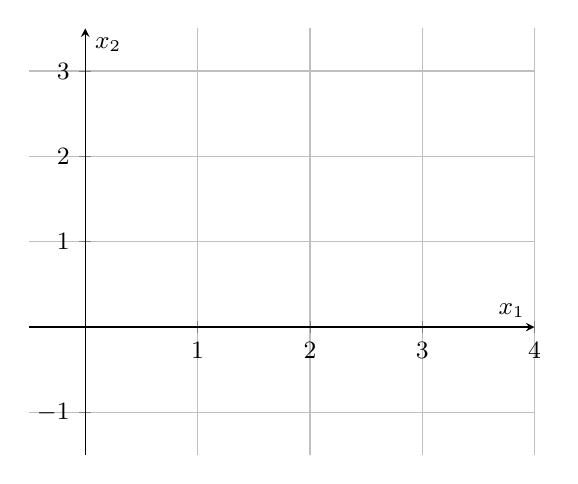
\begin{tikzpicture}
  \begin{axis}[
    width=8cm, height=7cm,
    xmin=-0.5, xmax=4,
    ymin=-1.5, ymax=3.5,
    xlabel={$x_1$}, ylabel={$x_2$},
    axis lines=center,
    grid=both,
    grid style={line width=0.3pt, draw=gray!30},
    major grid style={line width=0.5pt, draw=gray!50},
    xtick={0,1,...,4},
    ytick={-1,0,...,3},
    tick label style={font=\small},
    label style={font=\small},
  ]
  \end{axis}
\end{tikzpicture}
\end{center}

  \item Classify the following points. Compute $z = w_1 x_1 + w_2 x_2 + b$ and deduce $\hat{y}$.

\vspace{0.5em}
\begin{center}
\renewcommand{\arraystretch}{1.8}
\begin{tabular}{ccccc}
\toprule
Point & $x_1$ & $x_2$ & $z = 2x_1 - 3x_2 + 1$ & $\hat{y}$ \\
\midrule
$P_1$ & 0 & 0 & & \\
$P_2$ & 1 & 1 & & \\
$P_3$ & 2 & 2 & & \\
$P_4$ & 3 & 1 & & \\
$P_5$ & 0 & 2 & & \\
\bottomrule
\end{tabular}
\end{center}

  \item We want point $Q = (1,\, 2)$ to be classified as class~$1$. Is this currently the case?
  If not, propose a new value for the bias $b$ only (keeping $w_1$ and $w_2$ unchanged) that achieves this.

  \vspace{3.5em}

\end{enumerate}

% =============================================================
\section{Forward Propagation in a 2-2-1 MLP}
% =============================================================

Consider the following 2-2-1 MLP (step activation for all neurons):

\vspace{0.8em}
\begin{center}
\begin{tikzpicture}[
  neuron/.style={circle, draw=mainblue, fill=lightblue, minimum size=1cm, thick, font=\small\bfseries},
  arr/.style={->, >=Stealth, thick, gray!70},
  lbl/.style={font=\footnotesize, midway, sloped, above}
]
  % Input neurons
  \node[neuron] (x1) at (0, 1.5) {$x_1$};
  \node[neuron] (x2) at (0,-1.5) {$x_2$};
  % Hidden neurons
  \node[neuron, fill=green!15, draw=green!50!black] (h1) at (4, 1.5) {$h_1$};
  \node[neuron, fill=green!15, draw=green!50!black] (h2) at (4,-1.5) {$h_2$};
  % Output neuron
  \node[neuron, fill=orange!15, draw=orange!70!black] (y)  at (8, 0)   {$\hat{y}$};

  % Connections input -> hidden
  \draw[arr] (x1) -- node[lbl]{$W^{(1)}_{11}=1$} (h1);
  \draw[arr] (x1) -- node[lbl, below]{$W^{(1)}_{21}=1$} (h2);
  \draw[arr] (x2) -- node[lbl]{$W^{(1)}_{12}=1$} (h1);
  \draw[arr] (x2) -- node[lbl, below]{$W^{(1)}_{22}=-1$} (h2);

  % Connections hidden -> output
  \draw[arr] (h1) -- node[lbl]{$W^{(2)}_{1}=1$} (y);
  \draw[arr] (h2) -- node[lbl, below]{$W^{(2)}_{2}=1$} (y);

  % Layer labels
  \node[above=0.5cm of x1,  font=\small\bfseries\color{darkgray}] {Input};
  \node[above=0.5cm of h1,  font=\small\bfseries\color{darkgray}] {Hidden};
  \node[above=0.5cm of y,   font=\small\bfseries\color{darkgray}] {Output};
\end{tikzpicture}
\end{center}

\vspace{0.6em}

The network parameters are:
\[
  W^{(1)} = \begin{pmatrix} 1 & 1 \\ 1 & -1 \end{pmatrix},
  \quad
  b^{(1)} = \begin{pmatrix} -1.5 \\ -0.5 \end{pmatrix},
  \qquad
  W^{(2)} = \begin{pmatrix} 1 \\ 1 \end{pmatrix},
  \quad
  b^{(2)} = -1.5.
\]

Hidden neuron $i$ computes $h_i = f\!\left(\sum_j W^{(1)}_{ij}\, x_j + b^{(1)}_i\right)$.

\begin{enumerate}[label=\textbf{\arabic*.}, leftmargin=*, itemsep=0.9em]

  \item Compute $h_1$, $h_2$, and $\hat{y}$ for each input below. Show all intermediate values.

\vspace{0.5em}
\begin{center}
\renewcommand{\arraystretch}{2}
\begin{tabular}{cc|cc|cc|cc}
\toprule
$x_1$ & $x_2$ & $z_1^{(1)}$ & $h_1$ & $z_2^{(1)}$ & $h_2$ & $z^{(2)}$ & $\hat{y}$ \\
\midrule
0 & 0 & & & & & & \\
0 & 1 & & & & & & \\
1 & 0 & & & & & & \\
1 & 1 & & & & & & \\
\bottomrule
\end{tabular}
\end{center}

  \item What logical function does this network implement? Justify.

  \vspace{3em}

  \item Interpret each hidden neuron geometrically: what linear boundary does $h_1$ (resp.\ $h_2$) define in the plane $(x_1, x_2)$? Write each boundary equation explicitly.

  \vspace{3.5em}

\end{enumerate}

% =============================================================
\section{Designing MLP Architectures}
% =============================================================

For each task below, propose a complete MLP architecture and compute the \textbf{total number of parameters} (weights + biases).

\vspace{0.6em}

\begin{tcolorbox}[exercisebox, title={Task A — Spam Detection}]
An email is described by \textbf{20 numerical features} (keyword frequencies, message length, etc.).
The goal is binary classification: \emph{spam} or \emph{not spam}.

\begin{enumerate}[label=\textbf{\alph*.}, leftmargin=*, itemsep=0.5em]
  \item Propose an architecture (number of layers, neurons per layer, output activation).
  \item Count the total number of parameters for your choice.
\end{enumerate}

\vspace{4cm}
\end{tcolorbox}

\vspace{0.8em}

\begin{tcolorbox}[exercisebox, title={Task B — Handwritten Digit Recognition}]
Grayscale images of size $28 \times 28$ pixels. The goal is to recognize digits $0$ through $9$.

\begin{enumerate}[label=\textbf{\alph*.}, leftmargin=*, itemsep=0.5em]
  \item How many input neurons are needed?
  \item How many output neurons, and what activation function?
  \item Propose an architecture with \textbf{one hidden layer of 128 neurons} and count its parameters.
\end{enumerate}

\vspace{4cm}
\end{tcolorbox}

\vspace{0.8em}

\begin{tcolorbox}[exercisebox, title={Task C — Open Question}]
A student proposes the following architecture for Task B:\\[4pt]
\quad $784$ inputs $\;\to\;$ hidden layer of $10$ neurons (ReLU) $\;\to\;$ $10$ outputs (Softmax).

\begin{enumerate}[label=\textbf{\alph*.}, leftmargin=*, itemsep=0.5em]
  \item Compute the total number of parameters of this network.
  \item Do you think this network is expressive enough for the task?
  Write 2--3 sentences to support your answer.
\end{enumerate}

\vspace{4cm}
\end{tcolorbox}

\end{document}
